%%
% Please see https://bitbucket.org/rivanvx/beamer/wiki/Home for obtaining beamer.
%%
%\documentclass[11pt,aspectratio=169]{beamer}
%\documentclass[11pt,aspectratio=169,xcolor={dvipsnames}]{beamer}

\documentclass[11pt,aspectratio=169,xcolor={dvipsnames},hyperref={pdftex,pdfpagemode=UseNone,hidelinks,pdfdisplaydoctitle=true},usepdftitle=false]{beamer}
\usepackage{presentation}


\title{Lecture 17: Taxes in the Q Theory}
\author{Juan Herre\~{n}o\\UCSD}
\date{2026}

% Enter presentation title to populate PDF metadata:
\newcommand{\Cov}{\text{Cov}_\lambda}
\newcommand{\El}{\mathbb{E}_\lambda}
\newcommand{\mm}{\text{{\fontfamily{qzc}\selectfont m}}}
\usepackage{cancel}
\usepackage{booktabs}
\begin{document}

\maketitle


\begin{frame}{Tax Policy in the Q Theory}
\begin{itemize}
\item Taxation of firms takes many forms
\item Tax policy can, in principle, be used as countercyclical policy
\item Examples of taxes/subsidies used
\begin{itemize}
\item Business profit taxes
\item Dividend taxes
\item Investment tax credits: Deduct a share of investment expenditures
\item Bonus depreciation: Increases the speed at which firms can deduct investment expenditures
\end{itemize}
\end{itemize}
\end{frame}


\begin{frame}{Bonus depreciation}
\begin{figure}
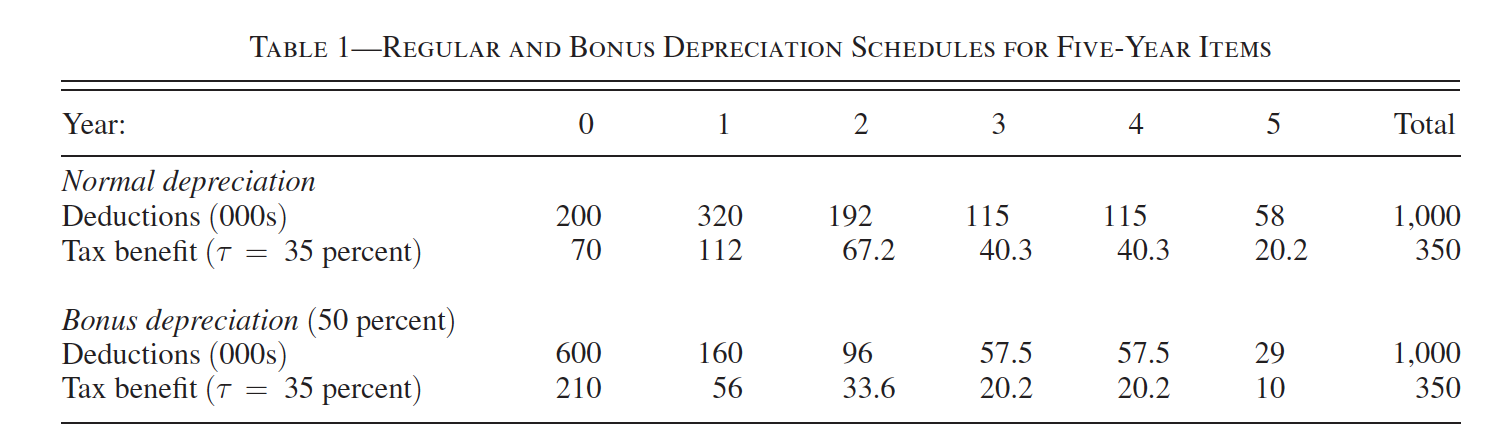
\includegraphics[scale=0.5]{Figures/bonus}\\
Source: Zwick and Mahon (2017)
\end{figure}
\end{frame}

\begin{frame}{Why bonus depreciation matters?}
Summers (1987, p. 29.5) states this most clearly: \textit{It is only because of discounting that depreciation schedules affect investment decisions”}
\begin{itemize}
\item Standard PV of deductions

\[z = \sum_{j=1}^R \frac{D^m_j}{(1+\pi)^j(1+r)^j} \]
\item Bonus depreciation

\[\lambda_t + (1-\lambda_t) z \]
\item PV of tax benefits due to bonus depreciation
\[\zeta_t  = (1-\tau_d) \tau_{\pi} (\lambda_t + (1-\lambda_t) z)  \] 
\end{itemize}
\end{frame}



\begin{frame}{Naive Model}
\begin{itemize}
\item Most of the theory you know is designed to understand non-durable goods
\item Capital is durable (not only capital. Durable consumption is an important part of household expenditures)
\item Standard supply and demand analysis may be arbitrarily uninformative if it ignores durability
\item Let's analyze that through an example
\end{itemize}
\end{frame}

\begin{frame}{Naive Model}
The world lasts for one period
\begin{itemize}
\item A firm that operates the production technology
\[y_t = k_t^{\alpha} \]
\item I am assuming the firm only uses capital for simplicity 
\item Firm profits are
\[\pi_t = y_t - q_t (1-\zeta_t)k_t \]
\item where $q_t$ is the relative price of capital
\item Profit maximization yields the condition \[k_t = \left(\frac{q_t (1-\zeta_t)}{\alpha}\right)^{-1/(1-\alpha)}\]
\item This is the capital demand equation.
\end{itemize}
\end{frame}

\begin{frame}{What is the slope of capital demand?}
In this interpretation, the capital demand elasticity $ \varepsilon^d = 1/(1-\alpha)$ should be between 5 and 10. Why?
\begin{itemize}
\item At the optimal capital demand, the share of profits to output is
\[\frac{\pi}{y} = 1-\alpha\]
\item Make sure you derive this at home. 
\item So if the profit share of income is between 10\% to 20\%, then the elasticity of capital demand is between 5 and 10.
\end{itemize}

\end{frame}

\begin{frame}{Capital supply and equilibrium}
Assume a very simple capital supply equation
\[k_t = q_t^{\xi}\]
\begin{itemize}
\item Equate demand and supply and find the following equilibrium relation

\[k_t  = \Theta (1-\zeta_t)^{-\frac{\xi}{(1-\alpha)\xi + 1}}\]
\item For an uninteresting constant $\Theta$
\item Take logs and do a first-order Taylor expansion around a point where $\zeta_t = \bar{\zeta}$
\[\log k_t \approx \log \bar{k} + \frac{\xi}{(1-\alpha)\xi + 1} \frac{1}{1-\bar{\zeta}} (\zeta_t - \bar{\zeta})\]
\end{itemize}
\end{frame}

\begin{frame}{What is the value of $\xi$}
Idea! Use knowledge on the profit share and the causal effects of $\zeta$ on $k$ to back out $\xi$.
\begin{itemize}
\item Rearrange using $\zeta = z \times \tau$
\[\Delta \log k_t \approx \frac{\xi}{(1-\alpha)\xi + 1} \frac{\tau}{1-\bar{z}\tau} \Delta z_t\]
\item Use the definition of supply and demand elasticities
\[\Delta \log k_t \approx \frac{\varepsilon^s \varepsilon^d}{\varepsilon^s + \varepsilon^d} \frac{\tau}{1-\bar{z}\tau} \Delta z_t\]
\item Zwick and Mahon '17 (on your reading list for next class) uses
$\Delta z \approx 0.05, \bar{z} \approx 0.9, \tau = 0.35, \Delta \log k_t \approx 0.17 $. Therefore:
\[\varepsilon^s \approx  \frac{-7 \varepsilon^d}{7 - \varepsilon^d}\]
\end{itemize}
\end{frame}

\begin{frame}{What is the value of $\xi$}
 If $\alpha = 0.8$ such that $\varepsilon = 5$.
\[\varepsilon^s \approx  \frac{-35}{2}\]
\begin{itemize}
\item A negative supply elasticity?!
\end{itemize}
 If $\alpha = 0.9$ such that $\varepsilon = 10$.
\[\varepsilon^s \approx 23\]
\begin{itemize}
\item Very large supply elasticity?
\end{itemize}
Apparently, little disagreement about the profit share changes inference by a lot!
\end{frame}

\begin{frame}{Should the profit share dictate the capital demand elasticity?}

\begin{itemize}
\item In this simple model, the shape of the production function, and nothing else, dictates the capital demand elasticity
\item Sensible assumptions when firms are buying/renting non-durable inputs
\item But firms are not supposed to maximize today's profits, but the PV of profits, and buying capital today has implications over those future profits.
\item Let's see what a model with durable inputs has to say about the shape of the capital demand equation
\end{itemize}

\end{frame}




\begin{frame}{Firm problem with taxes}
\[V_t = \max \sum_{j = 0}^{\infty}\Lambda_{t,t+j} \left( F(K_{t+j})(1-\tau^{\pi})(1-\tau^d) - I_t p_t (1-\zeta_t) \right)\]
subject to:

\[K_{t+1} = K_t(1-\delta) + I_t \]
\begin{itemize}
\item Simplifying assumption: Firm internalizes the PV of the deductions at time $t$. Common in key references, e.g. Hall and Jorgenson (1967), House and Shapiro (2008)
\item No labor explicitly. Easy to extend if labor market is spot, just more notation
\item Firm buys capital from outside producer at price $p$. Adjustment costs occur on that capital producing firm. Referred in the literature as \textit{external} adjustment costs
\end{itemize}
\end{frame}

\begin{frame}{Optimality conditions}
\[ q_t =  p_t (1-\zeta_t) \]
\[q_t = q_{t+1} \Lambda_{t,t+1} (1-\delta)  + \Lambda_{t,t+1} \left(F_k(K_{t+1})(1-\tau^{\pi})(1-\tau^d)  \right) \]
\begin{itemize}
\item Question: What is the effect of a change in $\zeta_t$?
\item Slightly simpler version of House and Shapiro (2008)
\item Pedagogical exercise: imagine a transient policy
\item The change in $\zeta$ does not last for long
\item Assume capital is highly durable ($\delta \approx 0$)
\item And firms are very forward looking ($\beta \approx 1$)
\end{itemize}
\end{frame}

\begin{frame}{Transitory Policy}
Let me assume that the change in $\zeta$ is transitory. $\zeta_{t+1} = \bar{\zeta}$. So the economy tomorrow will be close to the steady state.
\begin{itemize}
\item   $q_{t+1} \approx q^{ss}$
\item $\Lambda_{t,t+1} \approx \beta$
\item $\delta$ is small so that $\delta^2 \approx 0$ (For structures $\delta^2 = 0.0004$)
\end{itemize}
Transform:
\[q_t = q_{t+1} \Lambda_{t,t+1} (1-\delta)  + \Lambda_{t,t+1} \left(F_k(K_{t+1})(1-\tau^{\pi})(1-\tau^d)  \right) \]

into:

\[q_t = q^{ss} \beta (1-\delta)  + \beta \left(F_k(K_{t+1})(1-\tau^{\pi})(1-\tau^d) \right) \]

\end{frame}

\begin{frame}{Transitory Policy}
\[q_t = q^{ss} \beta (1-\delta)  + \beta \left(F_k(K_{t+1})(1-\tau^{\pi})(1-\tau^d)  \right) \]
In steady state:
\[q^{ss} = \frac{\beta}{1-\beta(1-\delta)}\left(F_k(K^{ss}) (1-\tau^{\pi})(1-\tau^d) \right) \]
Divide the first equation by the second one and rearrange

\[q_t \approx q^{ss} \left(\beta(1-\delta) + (1-\beta(1-\delta)) \frac{F_k(K_{t+1})}{F_k(K^{ss})} \right) \]
\begin{itemize}
\item For structures $1-\beta(1-\delta) = 0.052$
\item $K/Y = 4$, and $I/Y = 0.18$ , so $I/K = 0.045$
\item Imagine the reform had a large effect on investment. Second term still very small.
\end{itemize}
\end{frame}

\begin{frame}{Economics}
\begin{itemize}
\item On one side $q_t \approx q^{ss}$
\begin{itemize}
\item Capital is long lived. So the marginal benefit is dominated by stream of future MPKs into the distant future. Those do not change much with a temporary policy
\end{itemize}
\item On the other side
\[ q_t = p_t(1-\zeta_t)\]
\item the after-tax price of investment must be constant!
\item If investment subsidies go up, the pre-tax price must go up.
\item  The demand for capital does not depend on $I_t$. It is horizontal.
\item If capital is perfectly durable, firms are infinitely elastic on when to invest. If capital becomes cheaper today than tomorrow, I will invest today \textbf{rather than} tomorrow.
\item Note this argument is about the \textbf{timing} of investment expenditures, rather than the optimal size of the firm (which is given by steady state parameter values).
\end{itemize}
\end{frame}


\begin{frame}{With internal as opposed to external adjustment costs}

When adjustment costs are internal, the firm is the capital producer

\begin{itemize}
\item The firm will internalize that the effective cost of investment rises with the size of investment
\item The firm internalizes that investing more today reduces adjustment costs in the future
\end{itemize}
This is not an \textit{either or} question. In principle firms may buy capital from outside firms with increasing marginal costs, and face installation costs
\end{frame}

\begin{frame}{Firm problem with taxes}
\[V_t = \max \sum_{j = 0}^{\infty}\Lambda_{t,t+j} \left( F(K_{t+j})(1-\tau^{\pi})(1-\tau^d) - I_t(1-\zeta_t) - \frac{\varphi}{2}\left(\frac{I_{t+j}}{K_{t+j}}\right)^2 K_{t+j}\right)\]
subject to:

\[K_{t+1} = K_t(1-\delta) + I_t \]
\end{frame}

\begin{frame}{Optimality conditions}
\[\frac{I_t}{K_t} = \frac{1}{\varphi} (q_t - (1-\zeta_t)) \]
\[q_t = q_{t+1} \Lambda_{t,t+1} (1-\delta)  + \Lambda_{t,t+1} \left(F_k(K_{t+1})(1-\tau^{\pi})(1-\tau^d) + \frac{\varphi}{2}\left(\frac{I_{t+1}}{K_{t+1}}\right)^2 \right) \]
\end{frame}



\begin{frame}{Economics}
\begin{itemize}
\item On one side $q_t \approx q^{ss}$
\begin{itemize}
\item Capital is long lived. So the marginal benefit is dominated by stream of future MPKs into the distant future. Those do not change much with a temporary policy
\end{itemize}
\item On the other side \[\frac{I_t}{K_t} = \frac{1}{\varphi} (q_t - (1-\zeta_t)) \]
\begin{itemize}
\item The relative price of investment is decreasing from $(1-\zeta)$ to $(1-\zeta_t)$ when $\zeta$ increases
\item It must be that firms are investing more!
\[ \frac{d I/K}{d\zeta} = \frac{1}{\varphi}\]
\item Given our argument about $d q/d\zeta \approx 0$
\end{itemize}
\end{itemize}
\end{frame}






\begin{frame}{Economics}
Notice a couple of insights
\begin{itemize}
\item The reaction of investment to temporary tax policy depends critically on $\varphi$
\item The argument relies on a very horizontal demand curve for investment
\begin{itemize}
\item The marginal value of capital depend on stream of future MPKs
\item Changes in the after-tax relative price of investment in one period will convince firms to change the timing of their investments
\end{itemize}
\item $\frac{\partial I/K}{\partial q} = 1/\varphi$
\begin{itemize}
\item The responsiveness of $I$ to $\zeta$ depends on how costly is to build-up capital. The slope of capital supply is given by the adjustment cost function
\end{itemize}
\end{itemize}
\end{frame}

\begin{frame}{Numerical Results}
\begin{figure}
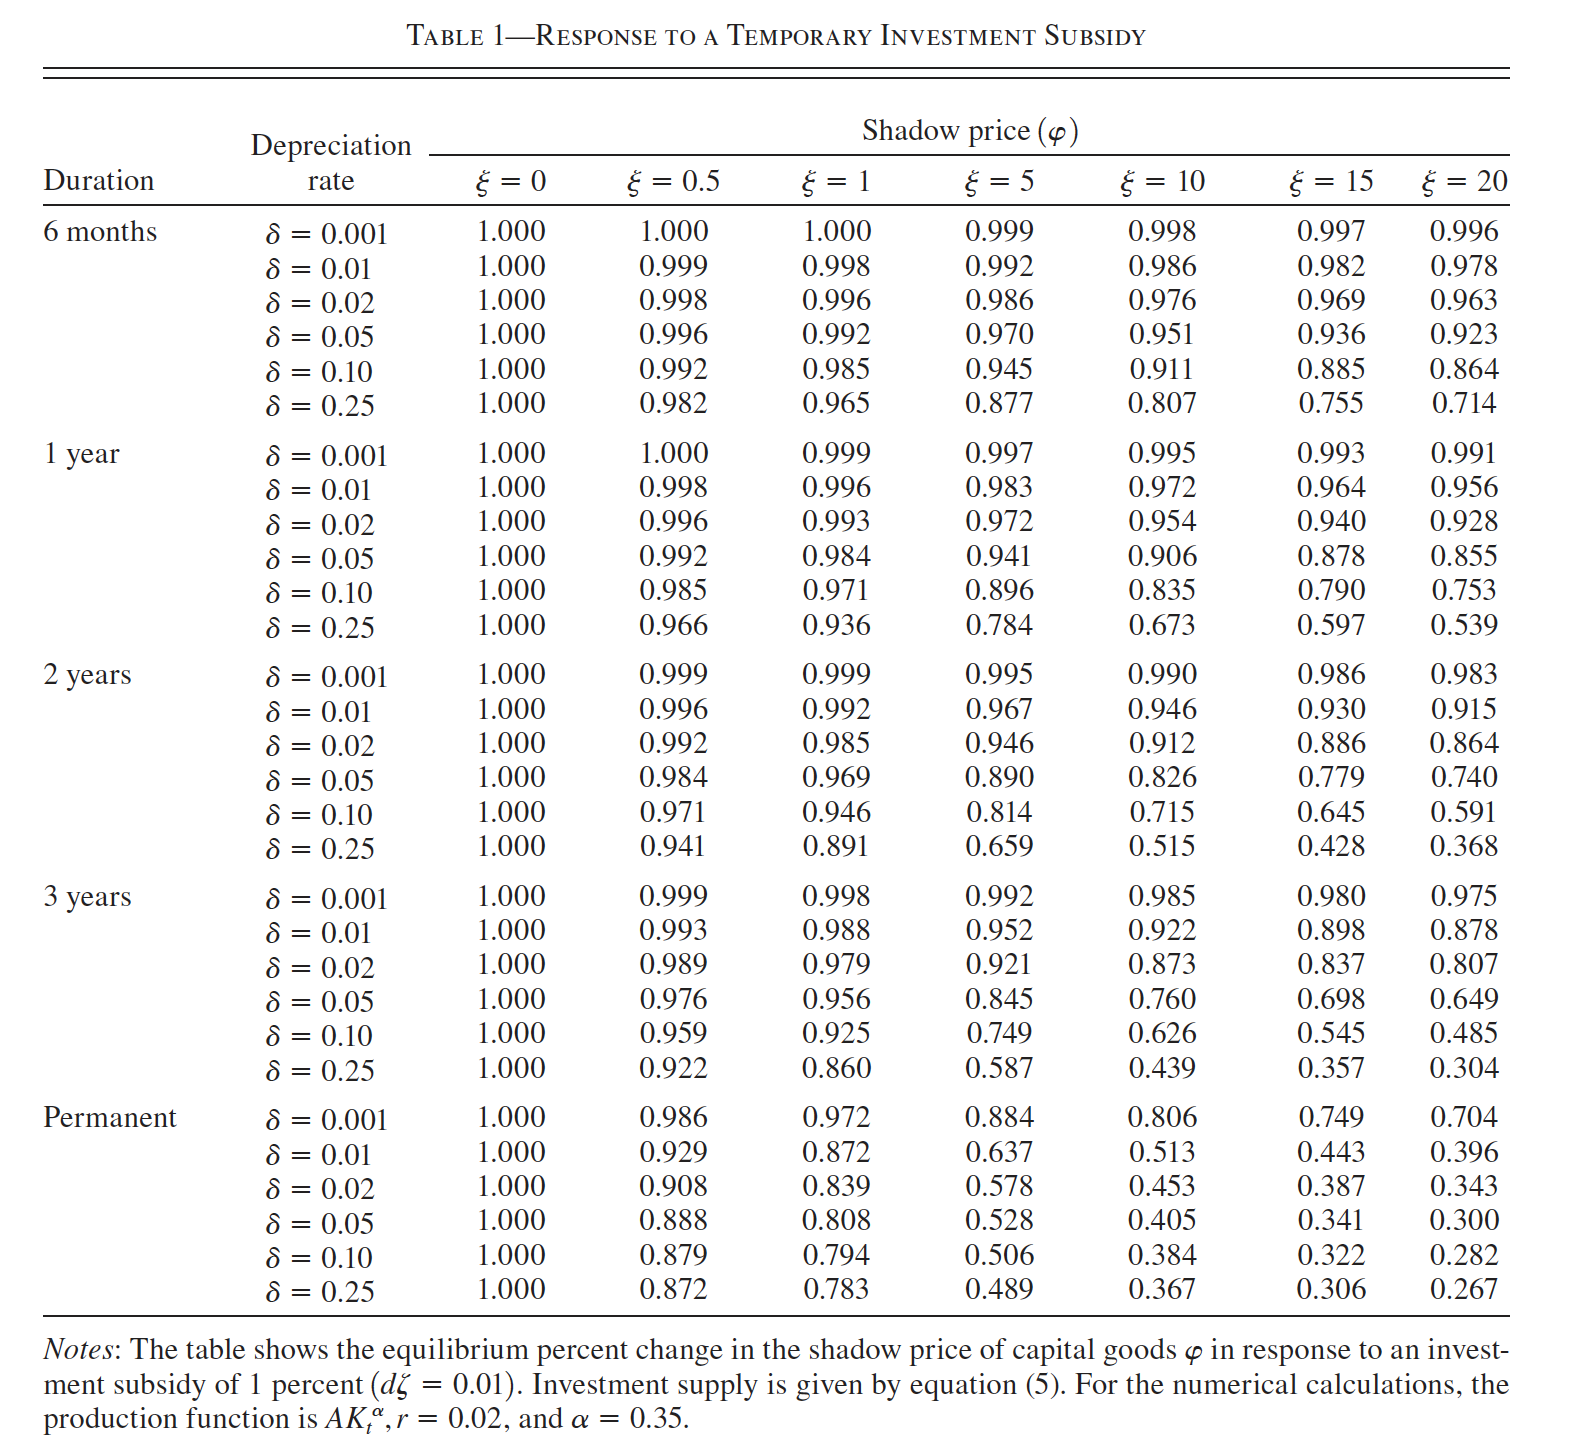
\includegraphics[height = 0.65\textheight]{Figures/house_shapiro}
\end{figure}
Source: House and Shapiro (2008). The effect on $q$ is 1 minus the effect on $\varphi$ (which in their notation is the shadow price of investment), and $\xi = (\delta \varphi)^{-1}$ in our notation.
\end{frame}

\end{document}



